\documentclass{beamer}
% Use DS9 global theme (includes pgfplots for visualization)
\usepackage{../../../shared/templates/ds9_theme}

% Configure image paths
\graphicspath{{../images/}}

% Title page configuration
\title[Intro to Physics and Kinematics]{PHYS11 CH:1-3}
\subtitle{Foundations of Physics, Motion, and Kinematics}
\author[Mr. Gullo]{Mr. Gullo}
\date[Jul 2025]{July 23, 2025}

\begin{document}
\frame{\titlepage}

\begin{frame}
\frametitle{Learning Objectives}
\begin{itemize}
    \item Define physics and its role as a fundamental science.
    \pause
    \item Differentiate between physical quantities, units, accuracy, and precision.
    \pause
    \item Distinguish between scalar quantities (distance, speed) and vector quantities (displacement, velocity).
    \pause
    \item Define acceleration as the rate of change of velocity.
    \pause
    \item Analyze and interpret motion using position-time and velocity-time graphs.
    \pause
    \item Understand the meaning of slope and area in motion graphs.
    \pause
    \item Identify and apply the kinematic equations for motion with constant acceleration.
\end{itemize}
\end{frame}

\section{The Language of Physics}

\begin{frame}
\frametitle{What is Physics?}
\begin{itemize}
    \item Physics is the most fundamental of the sciences, concerning itself with \alert{energy, matter, space and time}, and their interactions.
    \pause
    \item It provides the basis for all other sciences, including chemistry, biology, and geology.
    \pause
    \item \textbf{Modern Physics} includes two revolutionary theories:
    \pause
    \begin{itemize}
        \item \textbf{Relativity:} Describes how time, space, and gravity can be different for different observers.
        \pause
        \item \textbf{Quantum Mechanics:} Describes the behavior of subatomic particles.
    \end{itemize}
\end{itemize}
\end{frame}

\begin{frame}
\frametitle{Physical Quantities \& Units}
\begin{itemize}
    \item A \textbf{physical quantity} is a property of an object that can be measured (e.g., length, mass, time).
    \pause
    \item We use the \textbf{SI system} (metric system) for consistency.
    \pause
    \item The four fundamental units we will use are:
    \pause
    \begin{itemize}
        \item Length: \textbf{meter (m)}
        \pause
        \item Mass: \textbf{kilogram (kg)}
        \pause
        \item Time: \textbf{second (s)}
        \pause
        \item Electric Current: \textbf{ampere (A)}
    \end{itemize}
    \pause
    \item Unit conversions are essential for solving problems correctly.
\end{itemize}
\end{frame}

\begin{frame}
\frametitle{Accuracy vs. Precision}
\begin{description}
    \item[\textbf{Accuracy}] How close a measurement is to the correct or accepted value.
    \item[\textbf{Precision}] How close repeated measurements are to each other, regardless of their accuracy.
\end{description}
\vspace{1em}
An instrument can be precise without being accurate, or accurate without being precise. Our goal is to be both accurate and precise.
\end{frame}

\begin{frame}
\frametitle{Concept Visualization: Accuracy \& Precision}
To understand the difference between accuracy and precision, we can use the analogy of a dartboard.
\begin{itemize}
    \item \textbf{Accuracy} is hitting the bullseye.
    \item \textbf{Precision} is having all your darts land close together.
\end{itemize}
On the next slide, we will see four different scenarios.
\end{frame}

\begin{frame}
\frametitle{Visualizing Accuracy \& Precision}
\begin{figure}
    \centering
    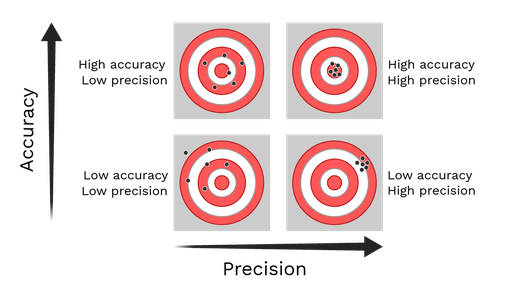
\includegraphics[width=0.8\linewidth]{phys11-accuracy-precision-targets.png}
    \caption{Four targets showing different combinations of accuracy and precision}
\end{figure}
\end{frame}

\section{Describing Motion}

\begin{frame}
\frametitle{Distance vs. Displacement}
\begin{itemize}
    \item \textbf{Distance} is a \alert{scalar} quantity. It is the total length of the path traveled.
    \pause
    \begin{itemize}
        \item Example: If you walk 5 meters east and 5 meters west, your distance traveled is 10 m.
    \end{itemize}
    \pause
    \item \textbf{Displacement} ($\Delta\vec{d}$) is a \alert{vector} quantity. It is the change in position from the start point to the end point.
    \pause
    \begin{itemize}
        \item $\Delta\vec{d} = \vec{d}_{final} - \vec{d}_{initial}$
        \pause
        \item In the example above, your displacement is 0 m because you ended where you started.
    \end{itemize}
\end{itemize}
\end{frame}

\begin{frame}
\frametitle{Concept Visualization: Distance vs. Displacement}
Imagine a person walking from their house to a store. The path they take might involve several turns.
\begin{itemize}
    \item The \textbf{distance} is the full length of the winding path they walked.
    \item The \textbf{displacement} is the straight-line distance and direction from the house to the store.
\end{itemize}
The next slide shows a map illustrating this.
\end{frame}

\begin{frame}
\frametitle{Visualizing Distance vs. Displacement}
\begin{figure}
    \centering
    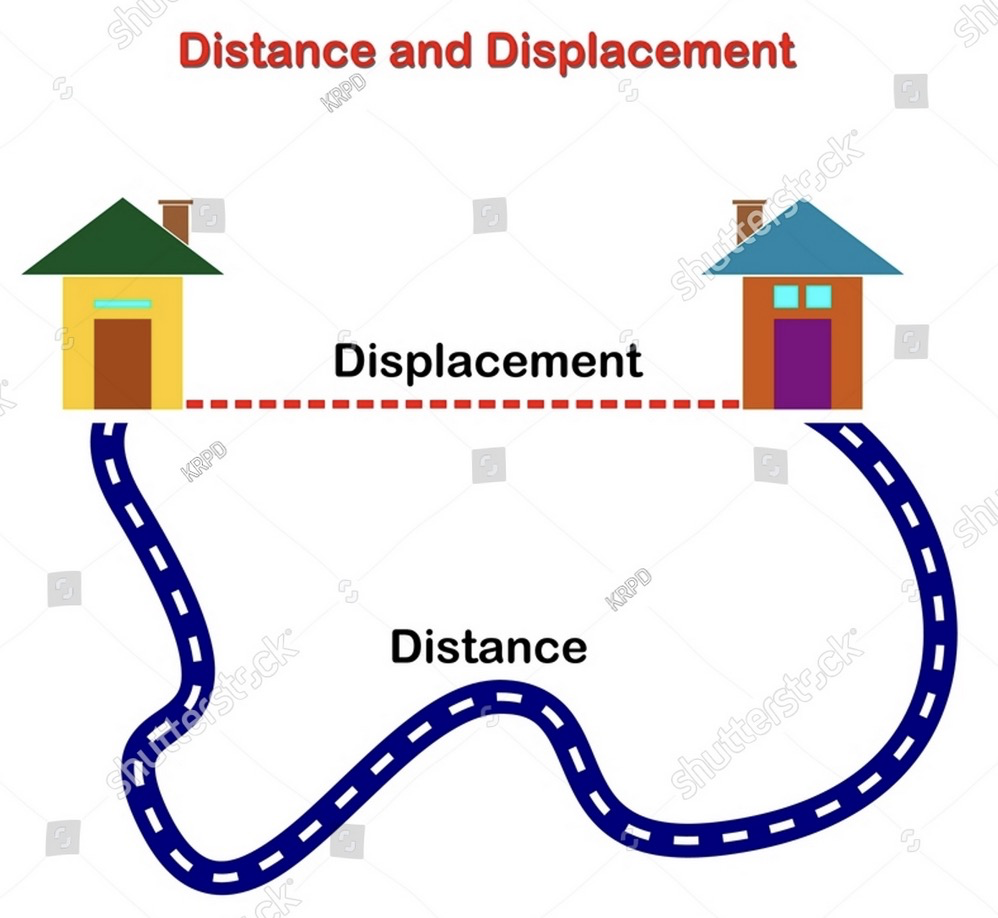
\includegraphics[width=0.5\linewidth]{phys11-distance-displacement-diagram.png}
    \caption{Map showing winding path (distance) vs. straight-line path (displacement)}
\end{figure}
\end{frame}

\begin{frame}
\frametitle{Speed vs. Velocity}
\begin{itemize}
    \item \textbf{Average Speed} is a \alert{scalar} quantity that describes the rate of covering distance.
    \pause
    \begin{itemize}
        \item $v_{avg} = \frac{\text{distance}}{\text{time}}$
    \end{itemize}
    \pause
    \item \textbf{Velocity} is a \alert{vector} quantity that describes the rate of displacement. It includes speed \textbf{and direction}.
    \pause
    \begin{itemize}
        \item $\vec{v}_{avg} = \frac{\text{displacement}}{\text{time}} = \frac{\Delta\vec{d}}{\Delta t}$
    \end{itemize}
    \pause
    \item \textbf{Instantaneous velocity} is the velocity at a specific moment in time.
\end{itemize}
\end{frame}

\section{Graphical Analysis of Motion}

\begin{frame}
\frametitle{Position vs. Time Graphs}
Graphs are a powerful way to visualize and analyze motion.
\pause
\begin{itemize}
    \item On a position-time (p-t) graph, the \textbf{y-axis} is position and the \textbf{x-axis} is time.
    \pause
    \item The \alert{slope} of the line on a p-t graph represents \alert{velocity}.
    \pause
    \begin{itemize}
        \item Slope $= \frac{\text{rise}}{\text{run}} = \frac{\Delta \text{position}}{\Delta \text{time}} = \text{velocity}$
    \end{itemize}
    \pause
    \item A \textbf{straight line} means constant velocity.
    \pause
    \item A \textbf{curved line} means changing velocity (acceleration).
\end{itemize}
\end{frame}

\begin{frame}
\frametitle{Visualizing Constant Velocity (p-t Graph)}
Let's visualize an object moving at a constant, positive velocity. The p-t graph will be a straight line with a positive slope. The value of that slope is the object's velocity.
\end{frame}

\begin{frame}
\frametitle{Position vs. Time Graph (Constant Velocity)}
\begin{figure}
\begin{tikzpicture}
\begin{axis}[
    width=\textwidth,
    height=0.7\textheight,
    xlabel={Time (s)},
    ylabel={Position (m)},
    xmin=0, xmax=6,
    ymin=0, ymax=12,
    grid=major,
    axis lines=left,
    label style={font=\large},
    tick label style={font=\small},
]
\addplot[ds9blue, thick, line width=1.5pt] coordinates {(0, 2) (5, 12)};
\draw[ds9red, dashed] (2,6) -- (5,6);
\draw[ds9red, dashed] (5,6) -- (5,12);
\node[ds9red, right] at (5,9) {$\Delta d = 6$ m (rise)};
\node[ds9red, below] at (3.5,6) {$\Delta t = 3$ s (run)};
\node[ds9blue, above, rotate=45] at (2.5, 7) {Slope = v = $\frac{6 \text{ m}}{3 \text{ s}} = 2 \text{ m/s}$};
\end{axis}
\end{tikzpicture}
\end{figure}
\end{frame}

\begin{frame}
\frametitle{Velocity vs. Time Graphs}
We can also graph velocity against time.
\pause
\begin{itemize}
    \item On a velocity-time (v-t) graph, the \textbf{y-axis} is velocity and the \textbf{x-axis} is time.
    \pause
    \item The \alert{slope} of the line on a v-t graph represents \alert{acceleration}.
    \pause
    \begin{itemize}
        \item Slope $= \frac{\Delta \text{velocity}}{\Delta \text{time}} = \text{acceleration}$
    \end{itemize}
    \pause
    \item The \alert{area under the curve} of a v-t graph represents \alert{displacement}.
    \pause
    \begin{itemize}
        \item Area = velocity $\times$ time = displacement
    \end{itemize}
\end{itemize}
\end{frame}

\begin{frame}
\frametitle{Visualizing Constant Acceleration (v-t Graph)}
Let's visualize an object moving with constant, positive acceleration. The v-t graph will be a straight line with a positive slope.
\begin{itemize}
    \item The \textbf{slope} of this line is the acceleration.
    \item The \textbf{area} under this line is the total displacement.
\end{itemize}
\end{frame}

\begin{frame}
\frametitle{Velocity vs. Time Graph (Constant Acceleration)}
\begin{figure}
\begin{tikzpicture}
\begin{axis}[
    width=\textwidth,
    height=0.7\textheight,
    xlabel={Time (s)},
    ylabel={Velocity (m/s)},
    xmin=0, xmax=6,
    ymin=0, ymax=12,
    grid=major,
    axis lines=left,
    label style={font=\large},
    tick label style={font=\small},
]
\addplot[ds9blue, thick, line width=1.5pt] coordinates {(0, 2) (5, 12)};
\addplot[fill=ds9gold, opacity=0.3, domain=0:5] {2*x+2} \closedcycle;

\node[above, rotate=45, ds9blue] at (2,7) {Slope = a = 2 m/s$^2$};
\node at (2.5, 3) {Area = Displacement};
\end{axis}
\end{tikzpicture}
\end{figure}
\end{frame}

\section{Acceleration \& Kinematic Equations}

\begin{frame}
\frametitle{Acceleration}
\begin{itemize}
    \item \textbf{Acceleration} is the rate at which an object's velocity changes. It is a \alert{vector} quantity.
    \pause
    \item It is measured in meters per second squared (m/s²).
    \pause
    \item An object is accelerating if it is:
    \pause
    \begin{itemize}
        \item Speeding up
        \pause
        \item Slowing down (this is often called deceleration, but it's still acceleration, just in the opposite direction of velocity)
        \pause
        \item Changing direction
    \end{itemize}
    \pause
    \item The formula for average acceleration is:
    \[ \vec{a} = \frac{\Delta \vec{v}}{\Delta t} = \frac{\vec{v}_f - \vec{v}_0}{t_f - t_0} \]
\end{itemize}
\end{frame}

\begin{frame}
\frametitle{Essential Equations: The Kinematics}
These equations describe motion with \textbf{constant acceleration}.
\pause
\begin{columns}
\column{0.6\textwidth}
\begin{enumerate}
    \item $\vec{v} = \vec{v}_0 + \vec{a}t$
    \pause
    \item $\Delta\vec{d} = \vec{v}_0 t + \frac{1}{2}\vec{a}t^2$
    \pause
    \item $\vec{v}^2 = \vec{v}_0^2 + 2\vec{a}\Delta\vec{d}$
    \pause
    \item $\Delta\vec{d} = \frac{\vec{v}_0 + \vec{v}}{2} t$
\end{enumerate}
\column{0.4\textwidth}
\pause
\textbf{Variables}:\\
$\Delta\vec{d}$: displacement (m)\\
$t$: time (s)\\
$\vec{a}$: acceleration (m/s²)\\
$\vec{v}_0$: initial velocity (m/s)\\
$\vec{v}$: final velocity (m/s)
\end{columns}
\vspace{1em}
\pause
\alert{Note:} We often write these without vector arrows in 1D problems, using +/- signs for direction.
\end{frame}

\section{Problem Solving}

\begin{frame}
\frametitle{The GUESS Method}
To solve physics problems consistently, we will use the \textbf{GUESS} method.
\pause
\begin{description}
    \item[\alert{G} - Givens] List all known quantities from the problem, with variable symbols and units.
    \pause
    \item[\alert{U} - Unknown] Identify the quantity you need to find.
    \pause
    \item[\alert{E} - Equation] Select the physics equation that relates your givens and unknown.
    \pause
    \item[\alert{S} - Substitute] Plug the known values (with units) into the equation.
    \pause
    \item[\alert{S} - Solve] Calculate the result, ensuring correct units and significant figures.
\end{description}
\pause
This structured approach helps prevent mistakes and makes your work easy to follow.
\end{frame}

\begin{frame}
\frametitle{I Do: Calculating Average Acceleration}
\begin{block}{Problem (12, p. 6)}
The driver of a sports car traveling at 10.0 m/s steps down hard on the accelerator for 5.0 s and the velocity increases to 30.0 m/s. What was the average acceleration of the car during the 5.0-s time interval?
\end{block}
\end{frame}

\begin{frame}
\frametitle{I Do: Calculating Average Acceleration - Solution Part 1}
\begin{block}{Solution using GUESS Method}
\begin{description}
    \item[\textbf{G - Givens:}]
        \begin{itemize}
            \item Initial velocity ($v_i$) = 10.0 m/s
            \item Final velocity ($v_f$) = 30.0 m/s
            \item Time interval ($t$) = 5.0 s
        \end{itemize}
    \item[\textbf{U - Unknown:}]
        \begin{itemize}
            \item Average acceleration ($a$) = ?
        \end{itemize}
    \item[\textbf{E - Equation:}]
        \[ a = \frac{\Delta v}{t} = \frac{v_f - v_i}{t} \]
\end{description}
\end{block}
\end{frame}

\begin{frame}
\frametitle{I Do: Calculating Average Acceleration - Solution Part 2}
\begin{block}{Solution using GUESS Method (continued)}
\begin{description}
    \item[\textbf{S - Substitute:}]
        \[ a = \frac{30.0 \, \text{m/s} - 10.0 \, \text{m/s}}{5.0 \, \text{s}} \]
    \item[\textbf{S - Solve:}]
        \[ a = \frac{20.0 \, \text{m/s}}{5.0 \, \text{s}} \]
        \[ a = 4.0 \, \text{m/s}^2 \]
\end{description}
\end{block}
\end{frame}

\begin{frame}
\frametitle{We Do: Finding Initial Speed}
\begin{block}{Problem (8, p. 4)}
A motorcycle moving at a constant velocity suddenly accelerates at a rate of 4.0 m/s² to a speed of 35 m/s in 5.0 s. What was the initial speed of the motorcycle?
\end{block}
\end{frame}

\begin{frame}
\frametitle{We Do: Finding Initial Speed - Setup}
\begin{block}{Let's use the GUESS Method}
\begin{description}
    \item[\textbf{G - Givens:}]
        \begin{itemize}
            \item Acceleration ($a$) = 4.0 m/s²
            \item Final velocity ($v_f$) = 35 m/s
            \item Time interval ($t$) = 5.0 s
        \end{itemize}
    \item[\textbf{U - Unknown:}]
        \begin{itemize}
            \item Initial velocity ($v_i$) = ?
        \end{itemize}
\end{description}
\end{block}
\end{frame}

\begin{frame}
\frametitle{We Do: Finding Initial Speed - Equation}
\begin{block}{Let's use the GUESS Method}
\begin{description}
    \item[\textbf{E - Equation:}]
        \[ v_f = v_i + at \]
        \alert{How do we rearrange this to solve for $v_i$?}
        \pause
        \[ v_i = v_f - at \]
\end{description}
\end{block}
\end{frame}

\begin{frame}
\frametitle{We Do: Finding Initial Speed - Solution}
\begin{block}{Let's use the GUESS Method}
\begin{description}
    \item[\textbf{S - Substitute:}]
        \alert{What values do we substitute into the equation?}
        \pause
        \[ v_i = 35 \, \text{m/s} - (4.0 \, \text{m/s}^2)(5.0 \, \text{s}) \]
    \item[\textbf{S - Solve:}]
        \[ v_i = 35 \, \text{m/s} - 20 \, \text{m/s} \]
        \[ v_i = 15 \, \text{m/s} \]
\end{description}
\end{block}
\end{frame}

\begin{frame}
\frametitle{You Do: Practice Problem}
\begin{block}{Problem (24, p. 12)}
How long does it take to accelerate from 8.0 m/s to 20.0 m/s at a rate of acceleration of 3.0 m/s²?
\end{block}
\vfill
\begin{alertblock}{Your Turn}
Use the GUESS method to solve the problem.
\begin{itemize}
    \item Identify your \textbf{Givens}.
    \item State the \textbf{Unknown}.
    \item Select the correct \textbf{Equation} and rearrange it.
    \item \textbf{Substitute} the values and \textbf{Solve}.
\end{itemize}
\end{alertblock}
\end{frame}

\section{Summary}

\begin{frame}
\frametitle{Lesson Summary}
\begin{itemize}
    \item Physics provides the fundamental rules for describing the universe.
    \pause
    \item Motion is described using \textbf{scalars} (distance, speed) and \textbf{vectors} (displacement, velocity, acceleration).
    \pause
    \item \textbf{Graphs} are a key tool for analyzing motion:
    \pause
        \begin{itemize}
            \item The slope of a position-time graph is \alert{velocity}.
            \pause
            \item The slope of a velocity-time graph is \alert{acceleration}.
            \pause
            \item The area under a velocity-time graph is \alert{displacement}.
        \end{itemize}
    \pause
    \item For motion with \textbf{constant acceleration}, we use the kinematic equations to relate displacement, velocity, acceleration, and time.
\end{itemize}
\end{frame}

\end{document}